\begin{activity} \label{A:7.1.2}  Shown below are two graphs depicting
  the velocity of falling objects.  On the left is the velocity of a
  skydiver, while on the right is the velocity of a meteorite entering
  the Earth's atmosphere.

\begin{center}
\begin{tabular}{cc}
\scalebox{0.75}{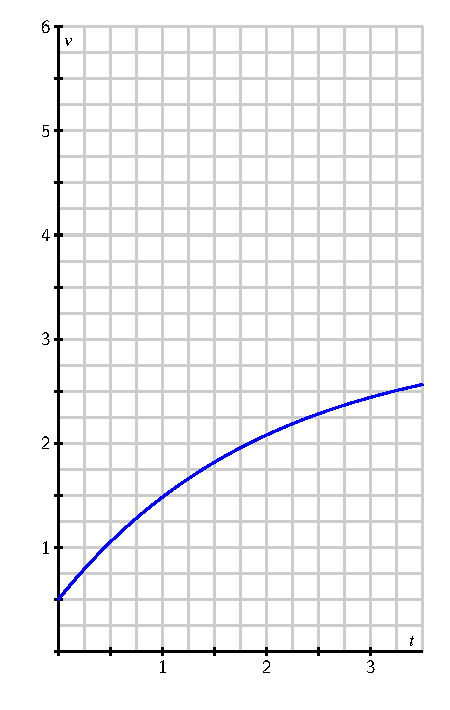
\includegraphics{figures/7_1_activity_0.eps}}
& 
\scalebox{0.75}{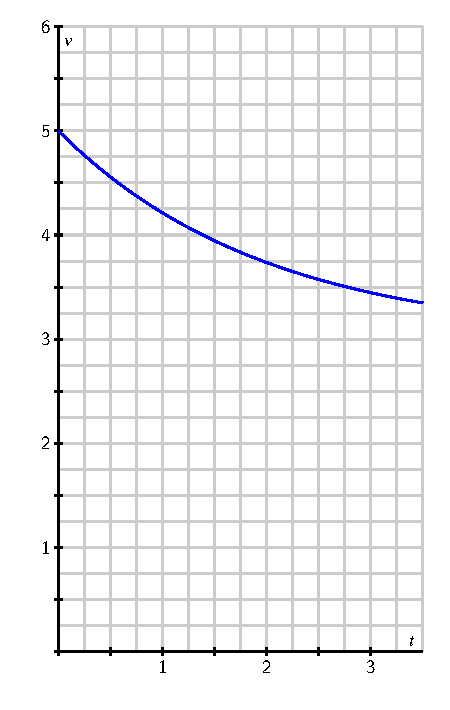
\includegraphics{figures/7_1_activity_1.eps}}
\\
Skydiver's velocity &
Meteorite's velocity \\
\end{tabular}
\end{center}
\ba
	\item Begin with the skydiver's velocity and use the given graph to measure the rate
          of change $dv/dt$ when the velocity is $v=0.5, 1.0, 1.5,
          2.0$, and $2.5$.  Plot your values on the graph below.  You
          will want to think carefully about this:  you are plotting
          the derivative $dv/dt$ as a function of {\em velocity}.

          \begin{center}
            \scalebox{0.65}{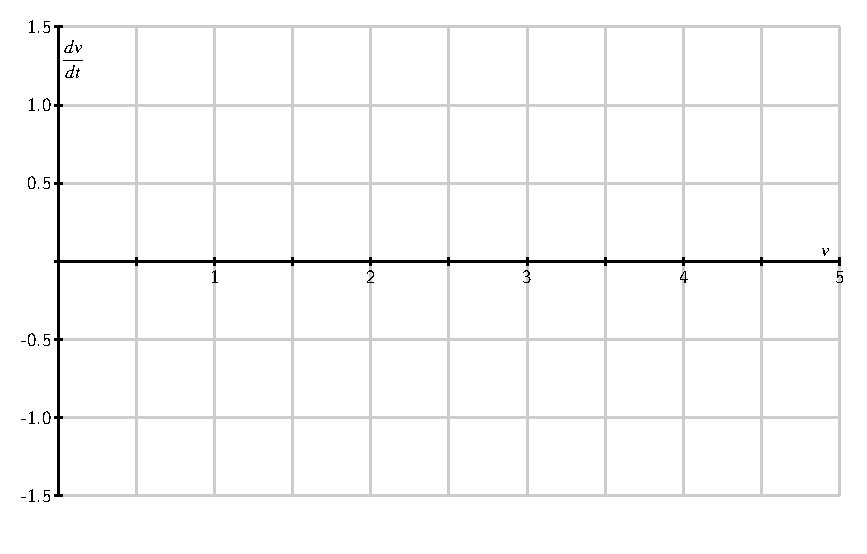
\includegraphics{figures/7_1_dataplot.eps}}
          \end{center}
        \item Now do the same thing with the meteorite's velocity:
          use the given graph to measure the rate of change $dv/dt$ when the velocity is
          $v=3.5,4.0,4.5$, and $5.0$.  Plot your values on the graph
          above. 
        \item You should find that all your points lie on a line.
          Write the equation of this line being careful to use proper
          notation for the quantities on the horizontal and vertical
          axes.
        \item The relationship you just found is a differential
          equation.  Write a complete sentence that explains its
          meaning. 
        \item By looking at the differential equation, determine the
          values of the velocity for which the velocity 
          increases.
        \item By looking at the differential equation, determine the
          values of the velocity for which the velocity 
          decreases.
        \item By looking at the differential equation, determine the
          values of the velocity for which the velocity 
          remains constant.

\ea
\end{activity}
\begin{smallhint}
\ba
	\item Small hints for each of the prompts above.
\ea
\end{smallhint}
\begin{bighint}
\ba
	\item Big hints for each of the prompts above.
\ea
\end{bighint}
\begin{activitySolution}
\ba
	\item Solutions for each of the prompts above.
\ea
\end{activitySolution}
\aftera